\startAnhang

\listofanhang
\clearpage

\anhang{Generierung synthetische Daten mithilfe des \textit{Omniverse Replicators} Quellcode}\label{anhang:replicator_code}
\footnote{Erstellung mit Unterstützung von ChatGPT-5 und Claude Sonnet 4}
\lstset{
  language=Python,
  basicstyle=\ttfamily\small,
  numbers=left,
  numberstyle=\tiny,
  stepnumber=1,
  numbersep=5pt,
  breaklines=true,        % Zeilenumbruch aktivieren
  breakatwhitespace=false, % nur an Leerzeichen umbrechen
  tabsize=4,
  showstringspaces=false,
  commentstyle=\color{gray}
}
\lstinputlisting{includes/code/replicator_script.py}

\anhang{Erstellung des Datensatzes für die Modelltrainings Quellcode}\label{anhang:datensatz_erstellen_code}
\lstset{
  language=Python,
  basicstyle=\ttfamily\small,
  numbers=left,
  numberstyle=\tiny,
  stepnumber=1,
  numbersep=5pt,
  breaklines=true,        % Zeilenumbruch aktivieren
  breakatwhitespace=false, % nur an Leerzeichen umbrechen
  tabsize=4,
  showstringspaces=false,
  commentstyle=\color{gray}
}
\lstinputlisting{includes/code/create_ds.py}

\anhang{Training der \ac{YOLO} Modelle Quellcode}\label{anhang:yolo_code}
\lstset{
  language=Python,
  basicstyle=\ttfamily\small,
  numbers=left,
  numberstyle=\tiny,
  stepnumber=1,
  numbersep=5pt,
  breaklines=true,        % Zeilenumbruch aktivieren
  breakatwhitespace=false, % nur an Leerzeichen umbrechen
  tabsize=4,
  showstringspaces=false,
  commentstyle=\color{gray}
}
\lstinputlisting{includes/code/train_yolo.py}

\anhang{Training of \ac{RT-DETR} Model Source Code}\label{anhang:rt_detr_code}
\lstset{
  language=Python,
  basicstyle=\ttfamily\small,
  numbers=left,
  numberstyle=\tiny,
  stepnumber=1,
  numbersep=5pt,
  breaklines=true,        % Zeilenumbruch aktivieren
  breakatwhitespace=false, % nur an Leerzeichen umbrechen
  tabsize=4,
  showstringspaces=false,
  commentstyle=\color{gray}
}
\lstinputlisting{includes/code/train_rtdetr.py}

\anhang{Evaluation der trainierten \ac{YOLO}-Modelle und des \ac{RT-DETR}-Modells Quellcode}\label{anhang:evaluation_models_code}
\lstset{
  language=Python,
  basicstyle=\ttfamily\small,
  numbers=left,
  numberstyle=\tiny,
  stepnumber=1,
  numbersep=5pt,
  breaklines=true,        % Zeilenumbruch aktivieren
  breakatwhitespace=false, % nur an Leerzeichen umbrechen
  tabsize=4,
  showstringspaces=false,
  commentstyle=\color{gray}
}
\anhangteil{Evaluation der \ac{YOLO}-Modelle auf synthetischen und realen Bilddaten Quellcode}
\label{anhang:evaluation_yolo_code}
\footnote{Erstellung mit Unterstützung von ChatGPT-5 und Claude Sonnet 4}
\lstinputlisting{includes/code/evaluate_yolo.py}

\anhangteil{Evaluation des \ac{RT-DETR}-Modells auf synthetischen und realen Bilddaten Quellcode}
\label{anhang:evaluation_rtdetr_code}
\footnote{Erstellung mit Unterstützung von ChatGPT-5 und Claude Sonnet 4}
\lstinputlisting{includes/code/evaluate_rtdetr.py}


\anhang{Metriken zur Evaluation der \ac{YOLO}-Modelle}\label{anhang:training_verlauf}
\anhangteil{Trainingsverlauf des Nano Modells}\label{anhang:training_nano}
\begin{figure}[htb]
\centering
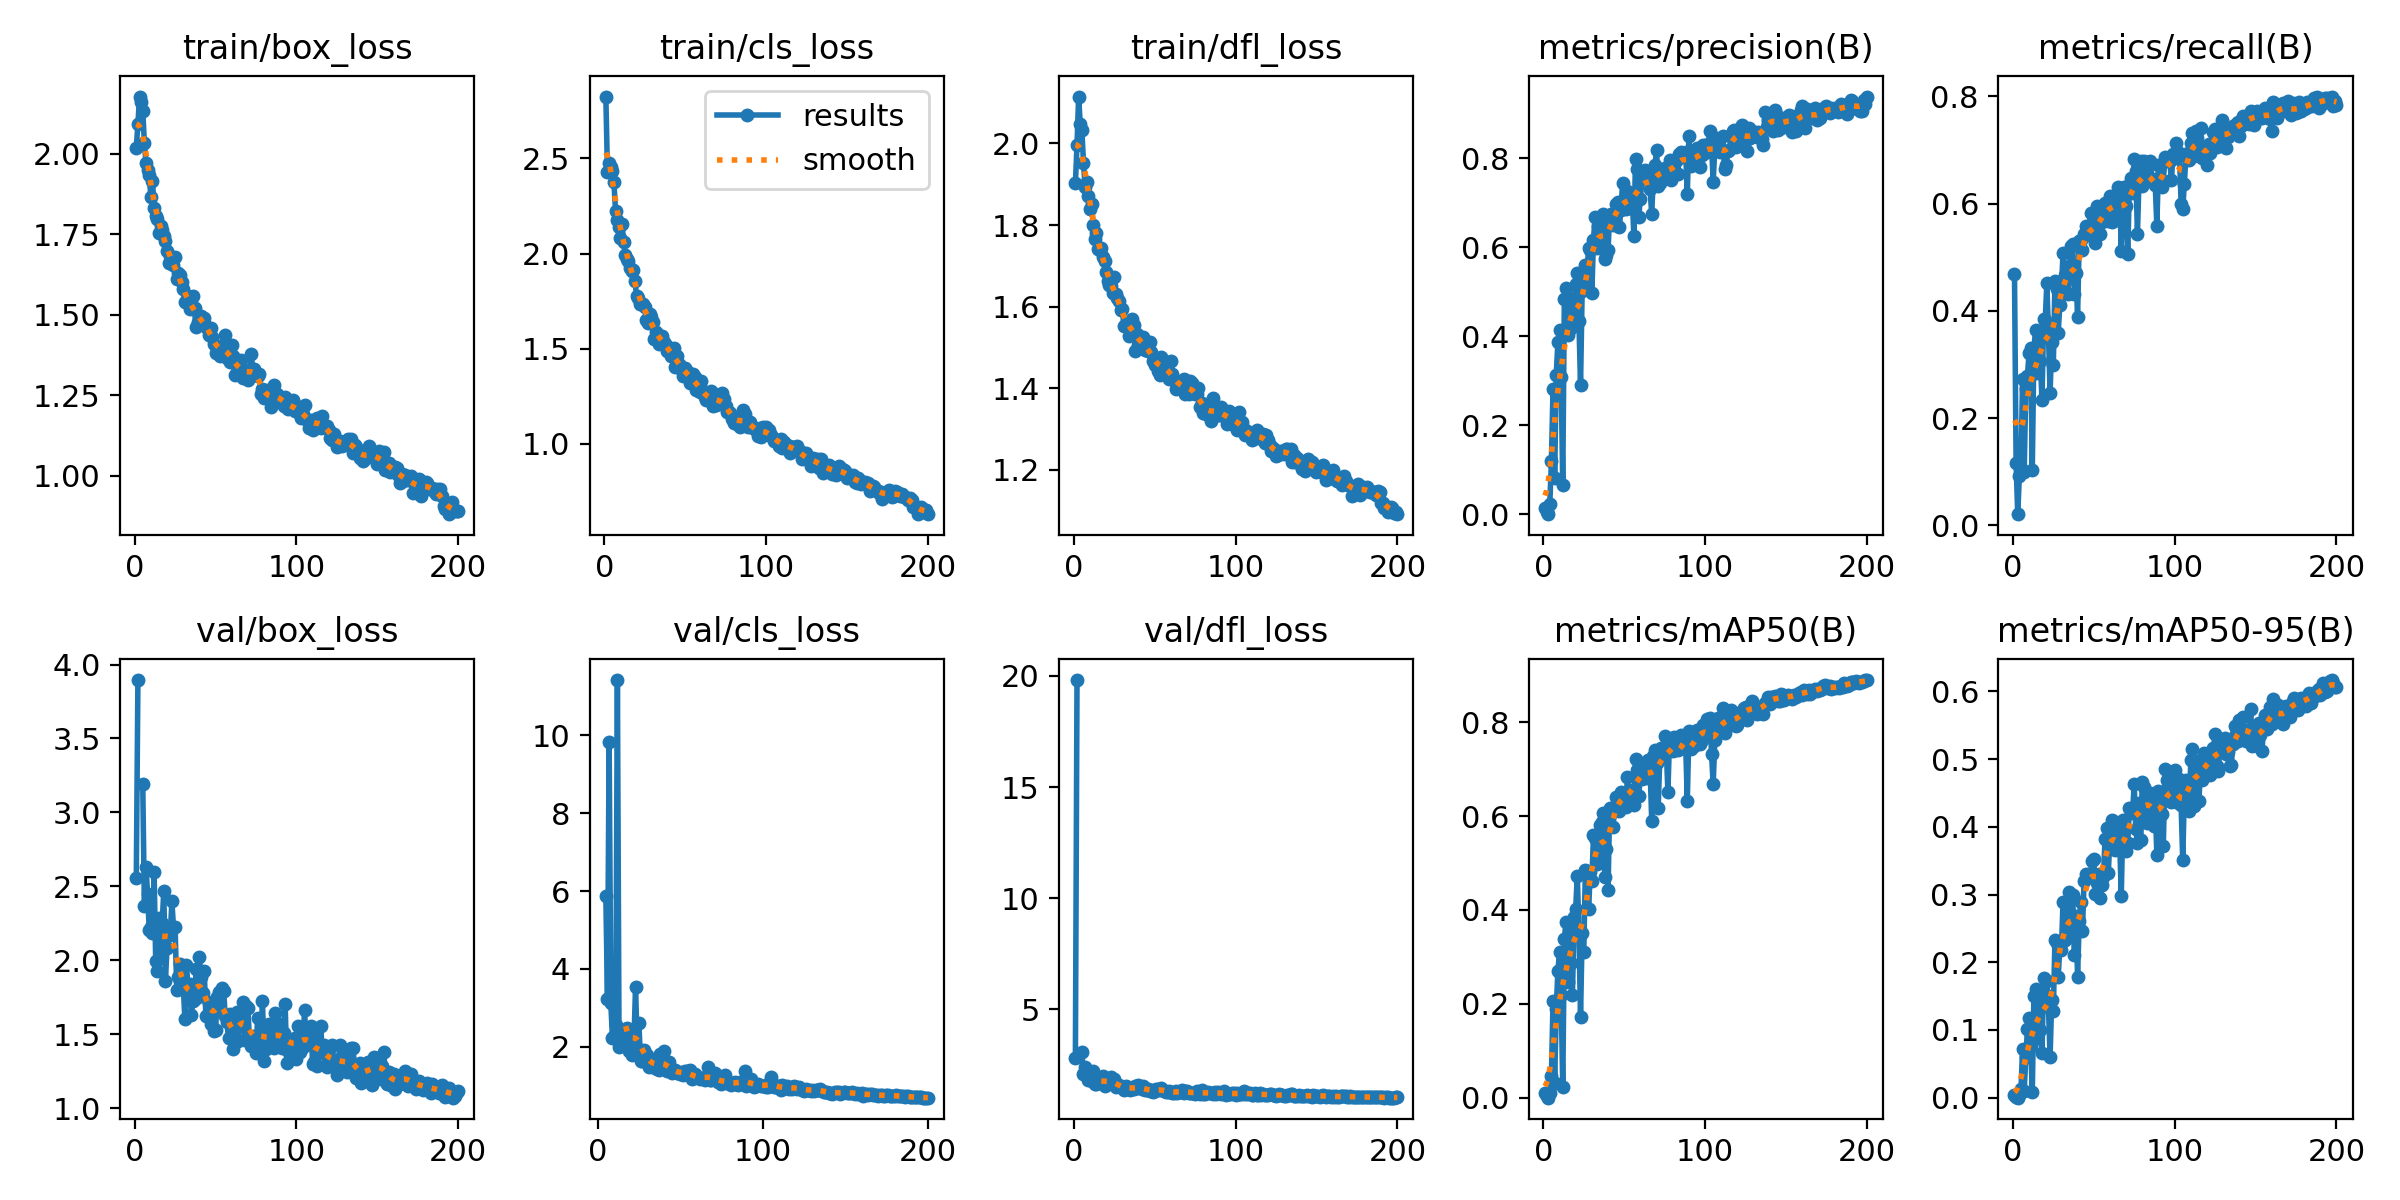
\includegraphics[width=0.9\linewidth]{graphics/yolo_eval/model_n/results.png}
\caption{Verlauf von Metriken während des Trainings des \ac{YOLO} Modells Nano}
\end{figure}

\anhangteil{Trainingsverlauf des Small Modells}\label{anhang:training_small}
\begin{figure}[htb]
\centering
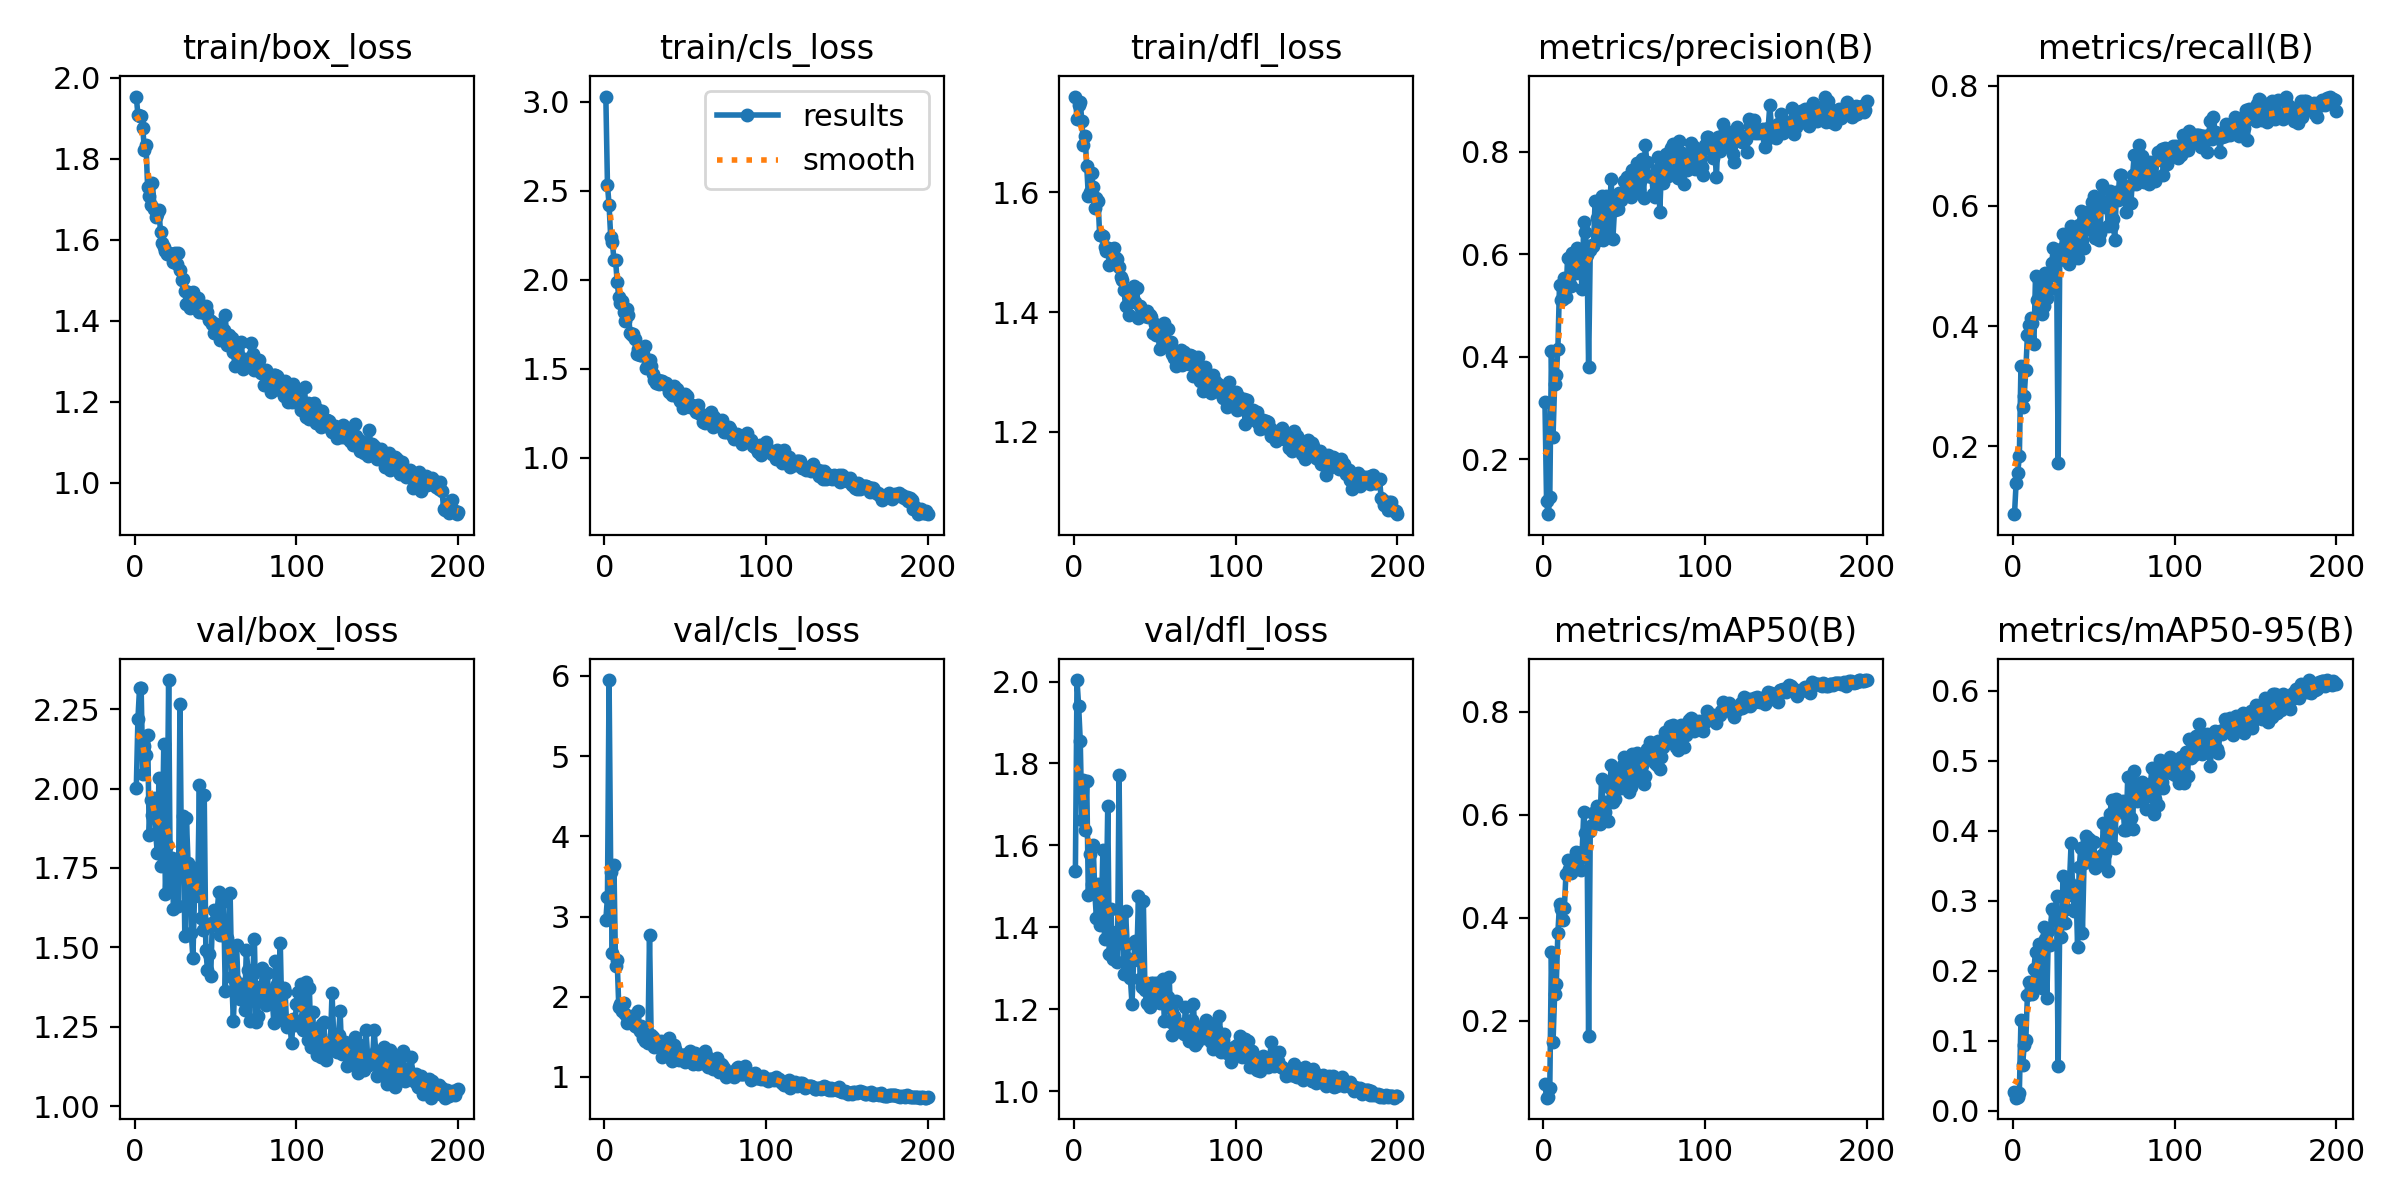
\includegraphics[width=0.9\linewidth]{graphics/yolo_eval/model_s/results.png}
\caption{Verlauf von Metriken während des Trainings des \ac{YOLO} Modells Small}
\end{figure}

\anhangteil{Precision-Recall-Kurve für das Small Modell}\label{anhang:pr_curve_small}
\begin{figure}[htb]
\centering
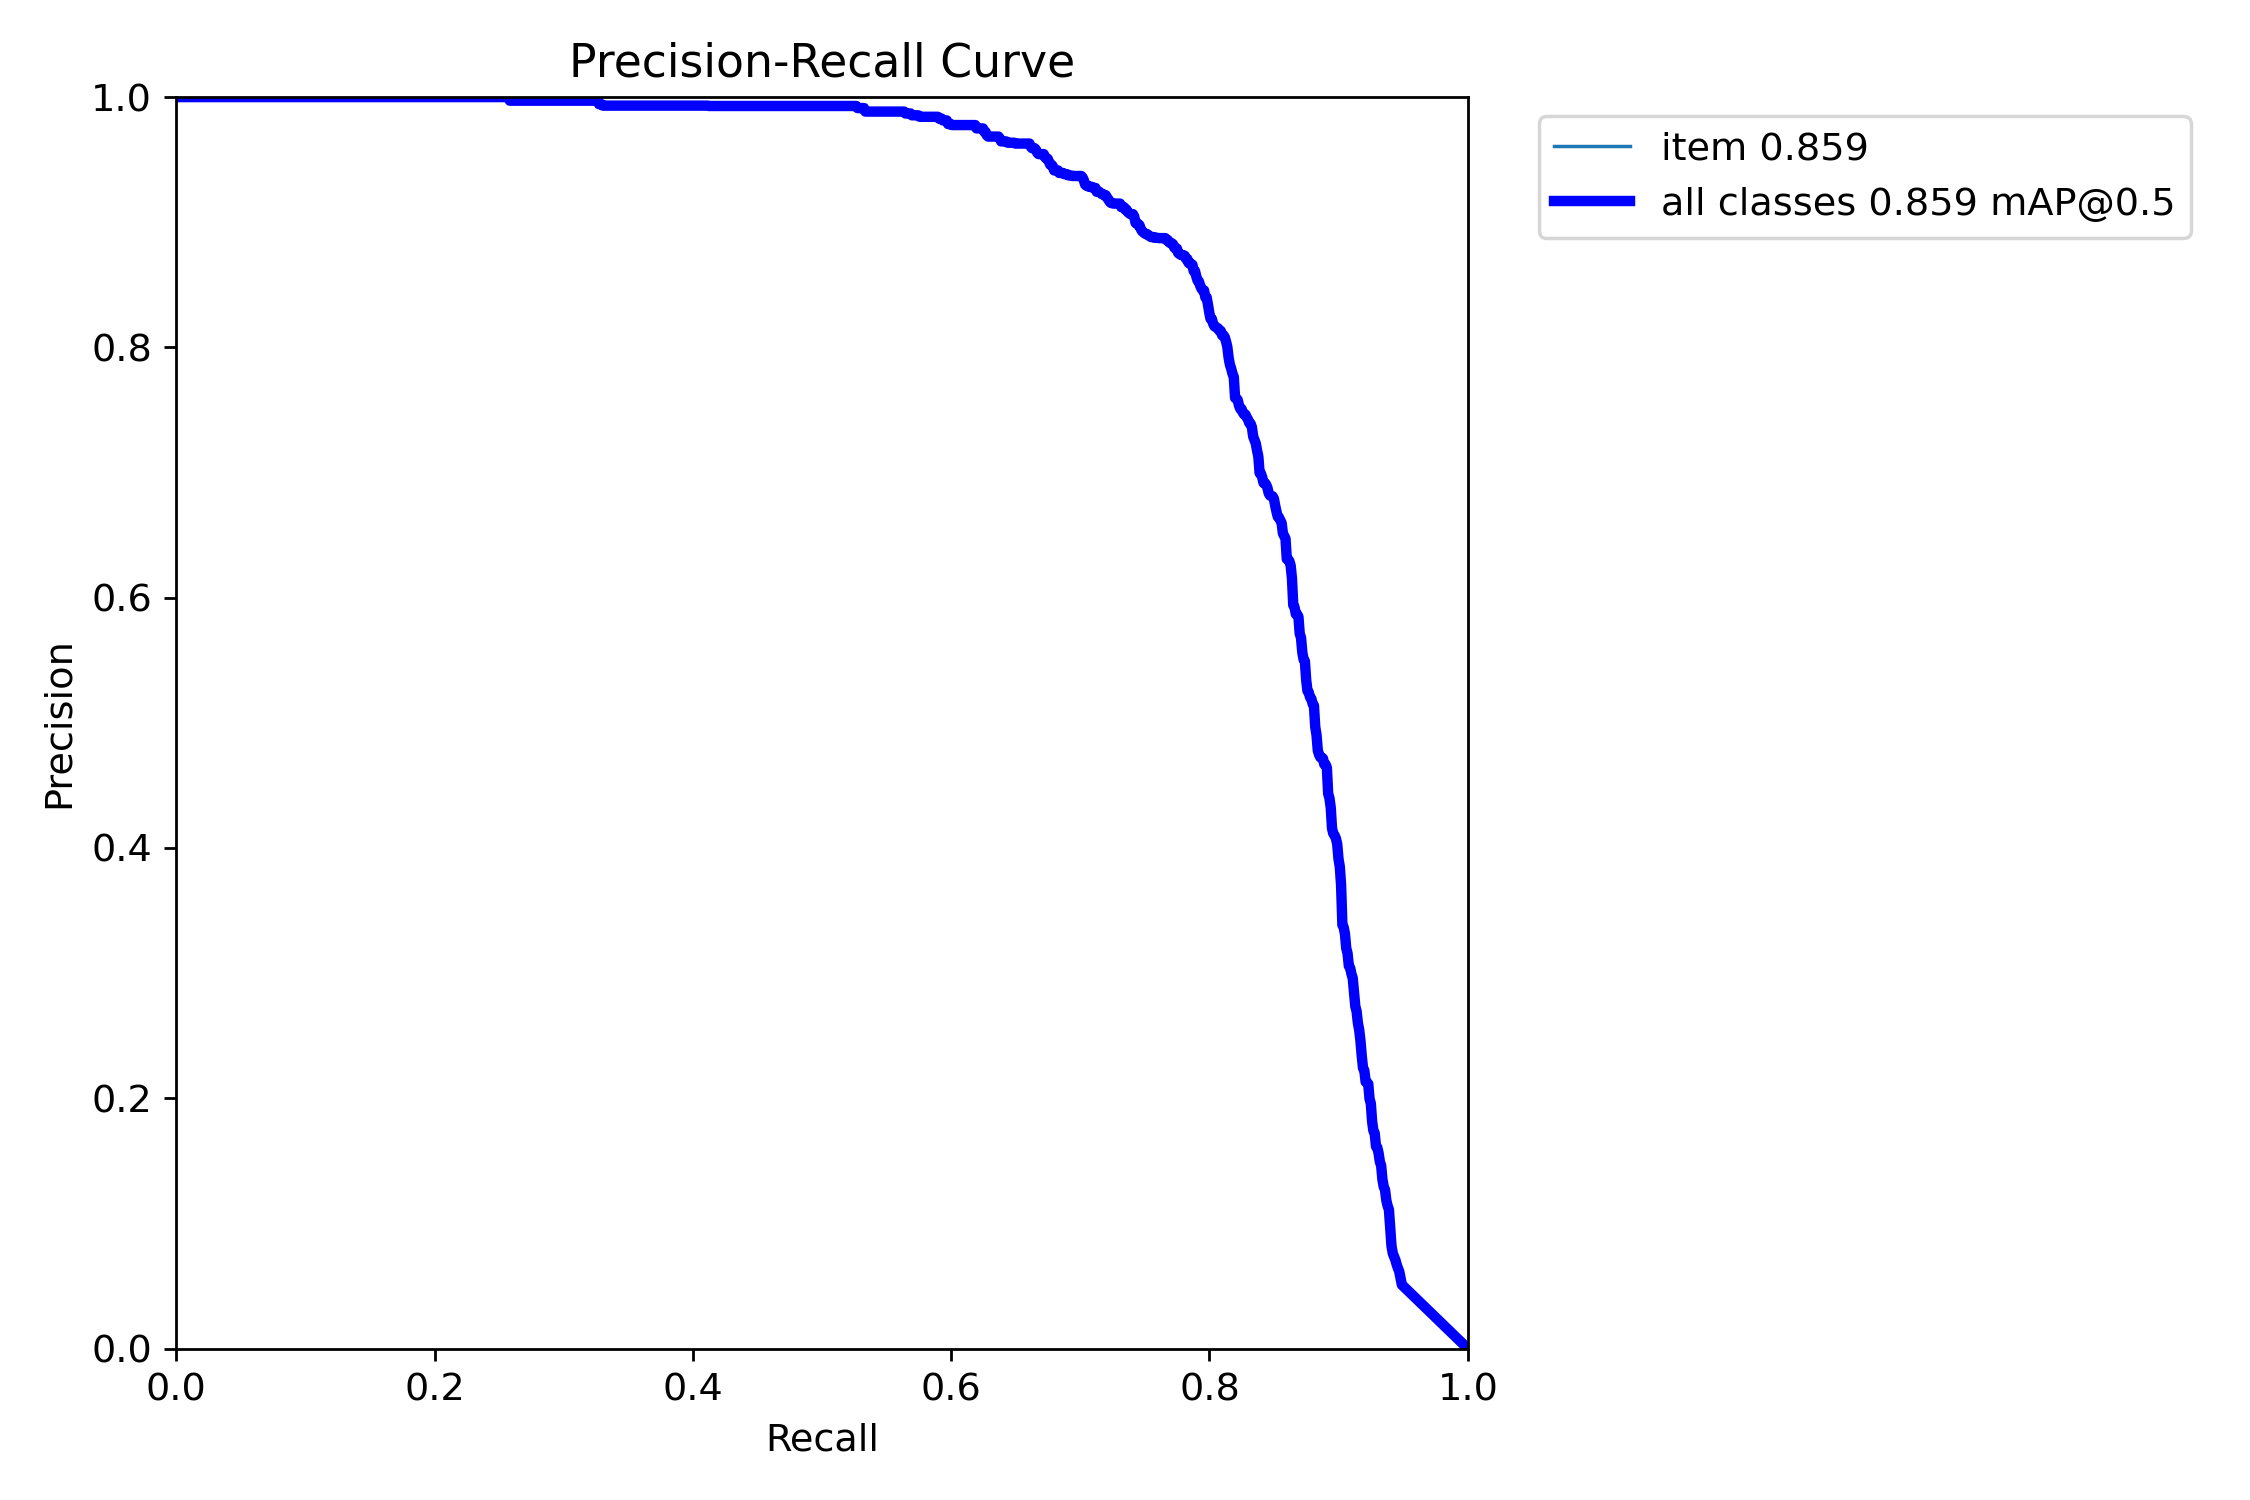
\includegraphics[width=0.9\linewidth]{graphics/yolo_eval/model_s/BoxPR_curve.png}
\caption{Precision-Recall-Kurve des \ac{YOLO} Small Modells}
\end{figure}